%!TEX root = main.tex
%\subsection{Decidability results}\label{sec:decidability}

%We investigate several decidability and asymptotic complexity questions concerning the synchronous semantics and synchronizability. 
%In this context, we consider finite-state message passing systems, where each process has a bounded number of local states.  
%We show that the reachability problem under the synchronous semantics, and checking $k$-synchronizability, are both decidable and PSPACE-complete. Therefore, even though these problems deal with asynchronous communicating systems, they have the same complexity as the reachability problem in a system using rendez-vous communication. Then, we give a class of systems for which the problem of checking whether there exists some $k$ such that they are  $k$-synchronizable is decidable. 
%Proofs of the results in this section can be found in Appendix~\ref{asec:decidability}.

Given a system $\mathcal{S}$, an integer $k$, and a local state $l$, \emph{the reachability problem under the $k$-synchronous semantics} asks whether there exists a $k$-synchronous execution of $\mathcal{S}$ reaching a configuration $(\vec{l},B)$ with $l=\vec{l}_p$ for some $p\in\<Pids>$. Theorem~\ref{th:main-verif} shows that checking $k$-synchronizability can be reduced to a reachability problem under the $k$-synchronous semantics. This reduction holds for arbitrary (infinite-state) systems, which implies that $k$-synchronizability can be checked using the existing assertion checking technology. Moreover, for finite-state systems, where each process has  a finite number of local states (message buffers can still be unbounded), it implies that checking this property is PSPACE-complete.

\vspace{-1mm}
\begin{theorem}\label{th:dec1}
For a finite-state system $\mathcal{S}$, the reachability problem under the $k$-synchronous semantics and the problem of checking $k$-synchronizability of $\mathcal{S}$ are decidable and PSPACE-complete.
\vspace{-1mm}
\end{theorem}

%\begin{figure}[t]
%\hspace{2cm}
%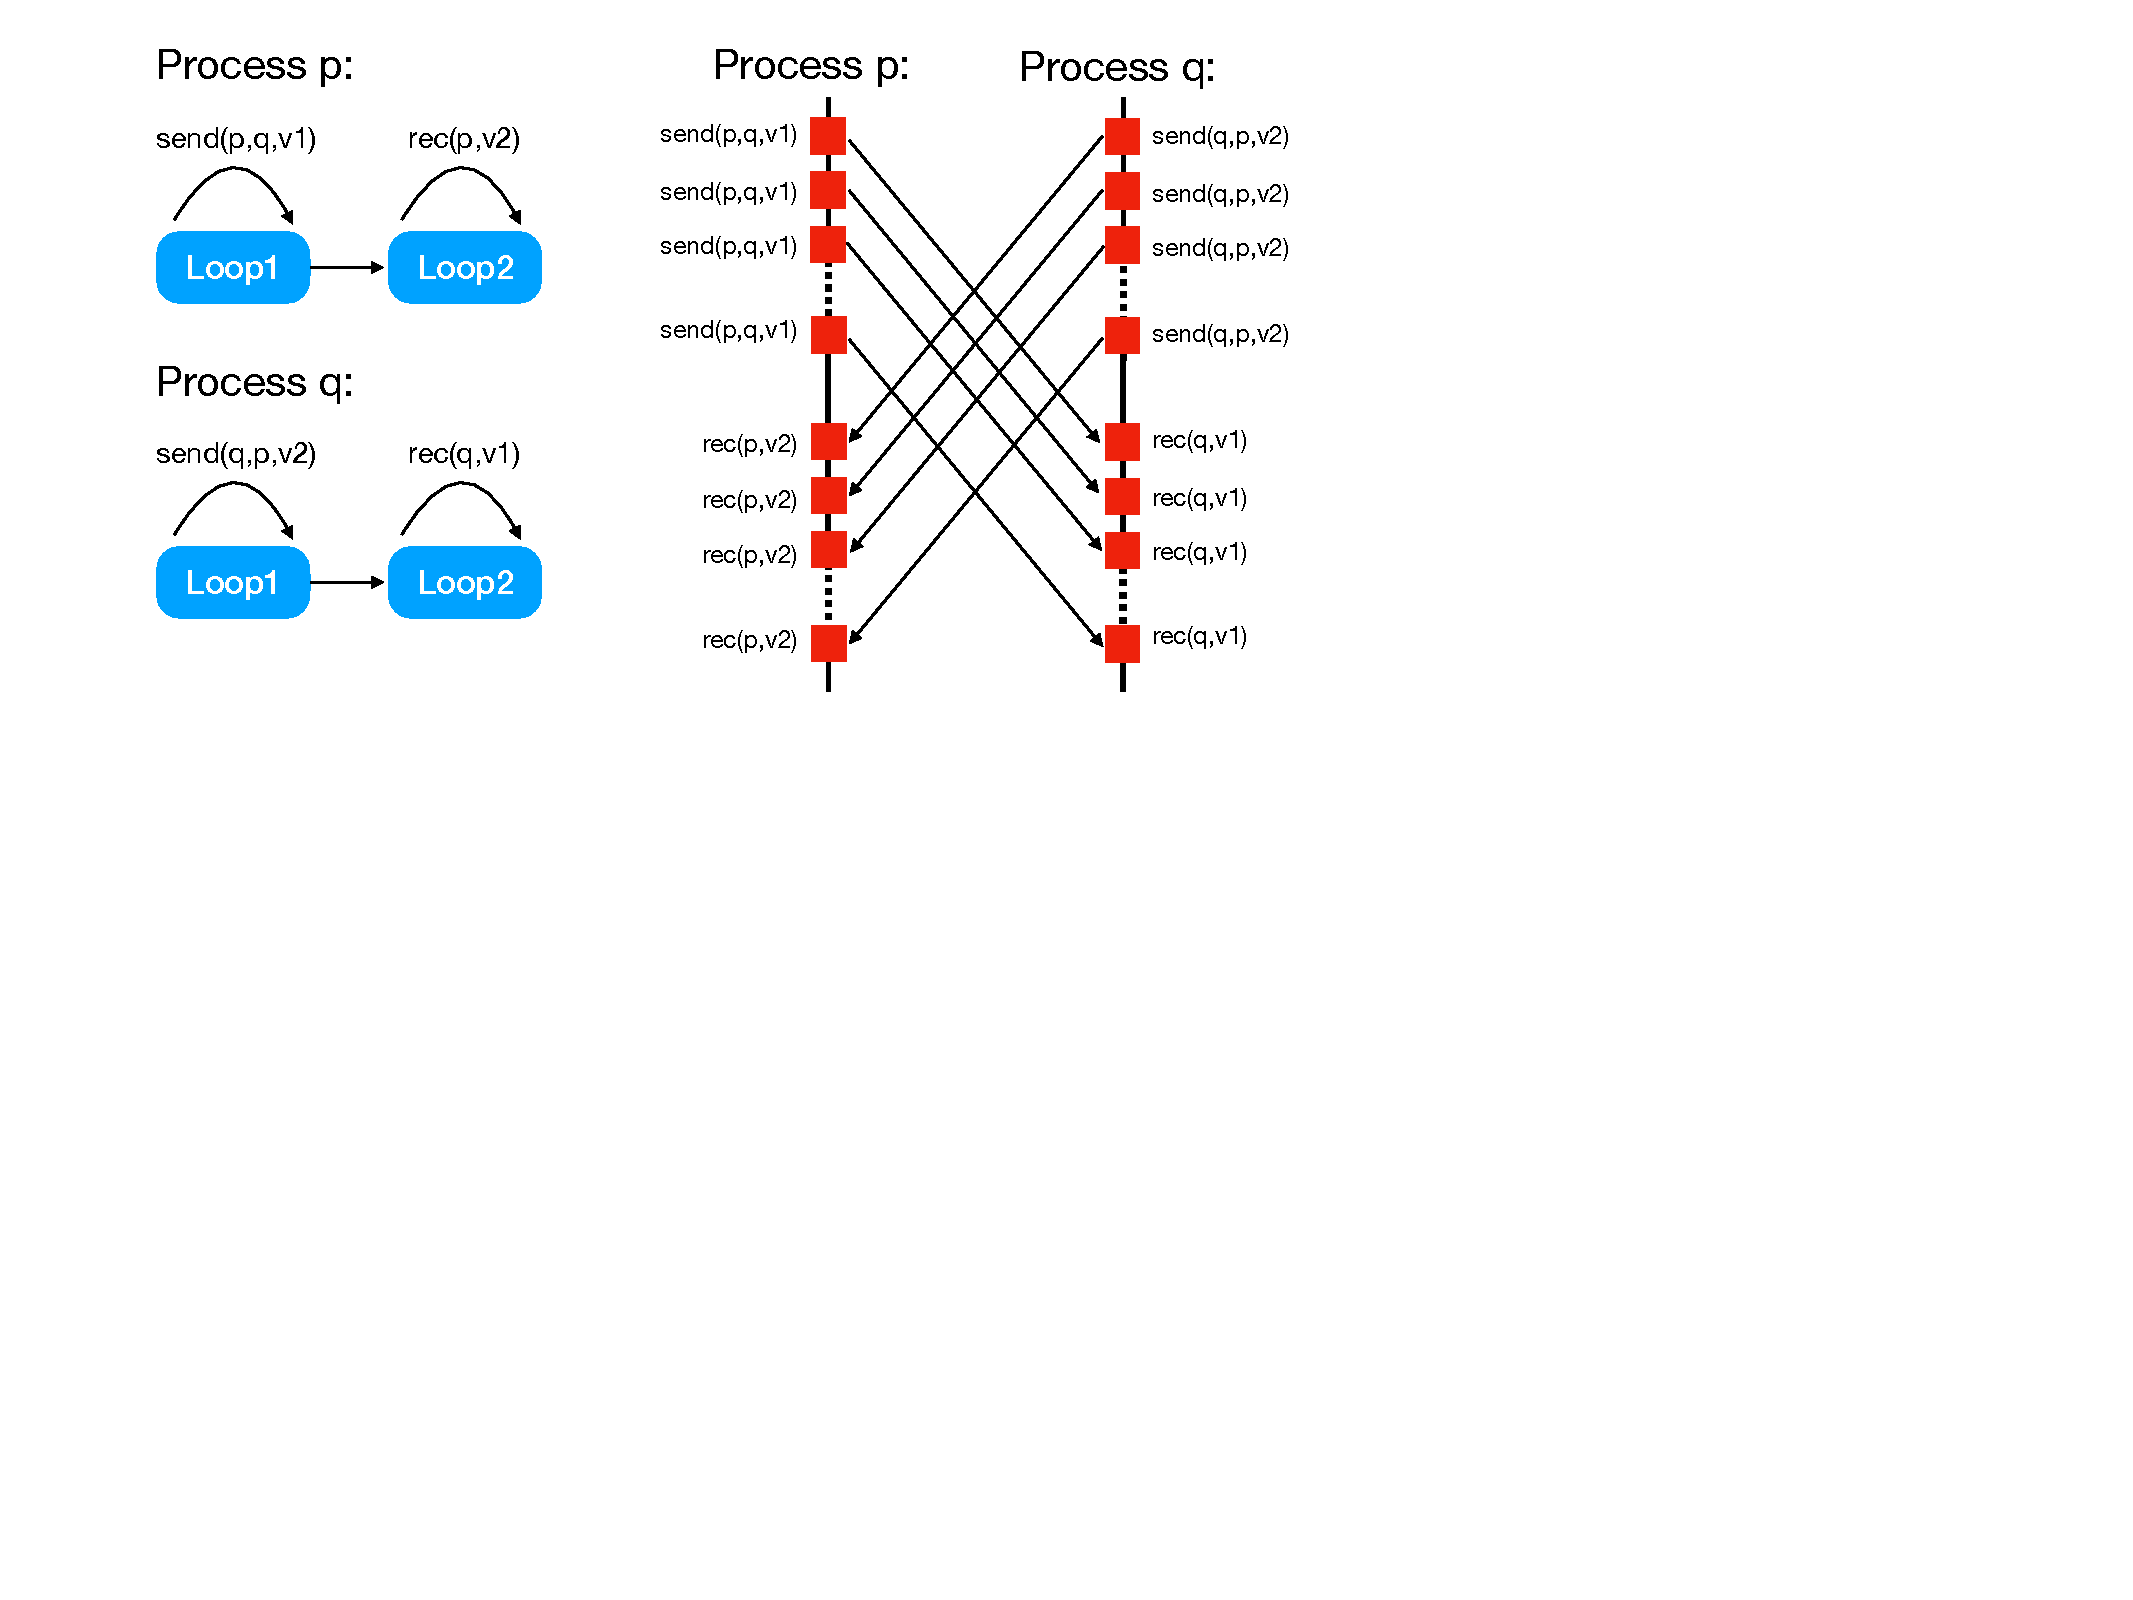
\includegraphics[width=7cm]{Ex-Decidability.pdf}
%\caption{An example of a system which is not $k$-synchronizable, for every $k$.}
%\label{fig:decid_ex}
%\vspace{-5mm}
%\end{figure}

%We now give a syntactical criterion that imposes an upper bound on the number $k$ for which a system could be $k$-synchronizable.
%In general, there are two reasons for which a system is not $k$-synchronizable, for every $k$. It either admits an execution with a bad conflict-graph cycle (e.g., the execution in Figure~\ref{fig:ex-rs-cycle}), or it admits executions with infinitely increasing conflict-graph cycles. If a system admits a bad conflict-graph cycle, then there exists a $k$ for which it can be shown to be non $k$-synchronizable (a coarse upper bound for $k$ is the length of the execution containing this cycle). The second case is exemplified by the system in Figure~\ref{fig:decid_ex}: the two loops in each process allow to create executions with unboundedly many send actions before any receive is enabled. However, the systems we have encountered in practice do not contain such scenarios. 
%
%In fact, the large majority of the processes composing practical systems, e.g., systems developed in the P language~\footnote{Available at \url{https://github.com/p-org}.}, perform a bounded number of consecutive receives, and a bounded number of sends before a receive. If all processes in the system would satisfy this constraint, then there exists a bound $k_s$ on the number of sends that are enabled before a receive, and a bound $k_r$ on the number of receives that are enabled before a send, which would imply that the system is $k$-synchronizable for some $k$ iff it is $k$-synchronizable for some $k\leq (k_s+k_r)\times |\<Pids>|$. However, there exist processes which don't satisfy this constraint, e.g., a consumer in a standard producer-consumer scenario and the process ${\tt Elevator}$ in Figure~\ref{fig:elevator}, which performs an unbounded number of consecutive receive actions. While in the first case, the system would be $1$-synchronous, in the second case, the unbounded number of receives is just an ``optimization'' that doesn't change the set of reachable local state vectors. The self loop where an unbounded number of messages ${\tt closeDoor}$ can be received from the ${\tt User}$ means that all these messages can be ignored since the door of the elevator is anyway closed. This unbounded interaction between ${\tt Elevator}$ and ${\tt User}$ will leave both processes in exactly the same state.
%% (${\tt Loop}$ for ${\tt User}$ and ${\tt Closed2}$ for ${\tt Elevator}$). 
%Removing this self loop and considering executions where the ${\tt User}$ sends exactly one message ${\tt closeDoor}$ instead of an unbounded sequence (before a message ${\tt openDoor}$) will allow to discover all the reachable local state vectors. Ignoring the self-loops in ${\tt Door}$ can be motivated in the same way. 
%%On the other hand, the process ${\tt Node}$ in Figure~\ref{fig:replication} doesn't satisfy this restriction, but this system is $k$-synchronizable where $k$ is the number of instances of ${\tt Node}$.
%
%Let $\mathcal{S}=((\<Lsts>_p,\delta_p,l_p^0)\mid p\in\<Pids>)$ be a message passing system. A process $p$ is called \emph{$k$-receive bounded} when it can perform at most $k$ consecutive receives, i.e., for every sequence $w\in (S\cup R)^*$ accepted by the labeled transition system $(\<Lsts>_p,\delta_p,l_p^0)$, there exists no decomposition $w=w_1\cdot w_2\cdot w_3$ where $w_2\in R^*$, and the length of $w_2$ is strictly bigger than $k$. A process $p$ is called \emph{$k$-send bounded} when it can perform at most $k$ consecutive sends before a receive, i.e., for every sequence $w\in (S\cup R)^*$ accepted by the labeled transition system $(\<Lsts>_p,\delta_p,l_p^0)$, there exists no decomposition $w=w_1\cdot w_2\cdot r\cdot  w_3$, where $r\in R$, $w_2\in S^*$, and the length of $w_2$ is strictly bigger than $k$.
%For instance, all the processes in the distributed commit protocol in Figure~\ref{fig:commit} are $2$-receive bounded and $2$-send bounded.
%%(more precisely, the manager is $2$-receive bounded and $2$-send bounded and the rest of the processes are $1$-receive bounded and $1$-send bounded). 
%%On the other hand, the process ${\tt Node}$  in Figure~\ref{fig:replication} is not $k$-receive bounded, for every $k$. 
%The system $\mathcal{S}$ is called \emph{flow-bounded} when there exists a constant $k$ such that every process $p\in\<Pids>$ is $k$-receive bounded and $k$-send bounded.
%Note that verifying flow-boundedness is reducible to a reachability problem for a single process and thus, decidable for finite-state processes.
%
%\begin{theorem}
%For a flow-bounded system $\mathcal{S}$, the problem of checking if there exists some $k$ such that $\mathcal{S}$ is $k$-synchronizable, is decidable.
%\end{theorem}
